

We enter now the core topic of the thesis. Most of the efforts during this PhD have been dedicated to the study of the Phase Problem 
for Bragg Coherent Diffraction Imaging using DL based approaches. Here I will discuss the main steps of this
journey, starting off from the analysis of the most relevant works in literature and concluding with our final version
of a DL model for highly strained particles. The latter has become the subject of an article, currently in preparation, 
entitled ``\textit{Phase Retrieval of Highly Strained Bragg Coherent Diffraction Patterns with Supervised Convolutional 
Neural Network}''. The process that led to the final version of the model will be unraveled, and particular attention
 will be given to elucidating the key steps and the critical issues encountered along the way. 

\section{State of the art}\label{chp:phasing_stateart}
In this paragraph I will focus on the state of the art for what concerns the Phase Retrieval of BCDI diffraction patterns with
deep-learning, tensor-computation and automatic differentiation methods. Conventional phase retrieval iterative algorithms 
are discussed in the introduction chapter as well as other approaches. \\
Given the relatively new development of neural networks and more specifically even more recent for BCDI phase retrieval, I will try
to give a chronological broad overview over many of the main works in the literature pointing out strengths and weaknesses.
The first work pioneering the field is ``Real-time coherent diffraction inversion using deep generative networks'' published
by Cherukara \textit{et. al} in 2018 \cite{cherukara_real-time_2018}. The paper presents two CNNs for the phase retrieval of small ($32\times32$ pixels) 2D 
simulated BCDI patterns, one predicting the support and the other the phase. A U-Net like architecture with 
encoder-decoder was implemented, and the model was trained for just 10 epochs in a supervised fashion with a cross-entropy loss function (see Appendix).
The results showed an excellent agreement between prediction and ground truth also in presence of relatively strong phases. 
The potential of this new approach for phase retrieval becomes immediately clear when considering the drastic reduction of
computational time and resources needed for the model inference. Once the model is trained, the reconstruction can be obtained
within few milliseconds on a desktop machine. In 2020 Scheinker and Pokharel proposed another approach \cite{scheinker_adaptive_2020}
that employs a CNN model for 3D diffraction patterns. The fundamental difference is that the object's support was defined 
by its surface only, as it is assumed to be \textit{compact} and \textit{homogeneous} inside. Moreover, the surface was
parametrized by spherical harmonics and the DL model was trained to predict 28 of the first even coefficients of the spherical
harmonics. The model architecture was therefore essentially different since, while the encoder is just transposed to a 3D 
one, the decoder is replaced by a flattening and dense layer with 28 different classes as output. The model showed good performance
on both simulated and experimental data, marking the first DL-based approach capable of real 3D BCDI phase retrieval.
In the same year, Wu and coauthors, \cite{Wu2021}, opted for an architecture made of a single encoder and two identical decoders for the prediction of 
amplitude and phase of single crystals from the central slice of the BCDI pattern. They conducted the study on simulated 
data and tested it on one experimental case as well. What is evident from their work is the winning combination of DL prediction
and iterative refinement. The speed and generalization capabilities of the CNN allows for fast and good estimations of the 
object's support and phase. In addition, the precise and well established iterative methods can bring this initial guess to a 
more polished and accurate solution in fewer cycles than without DL prediction. This successful combined approach has been 
later adopted in other works, ours included. In 2021 two important works were published. First, Chan \textit{et al.} in 
\cite{chan_rapid_2021} extended the encoder/2-decoders architecture to the 3D case. In their work they first created a 
``physics-informed'' training set obtained building particles by clipping planes from a cubic FCC structure of atomic 
positions, relaxing them with LAMMPS software for molecular dynamics and computing the BCDI pattern around the (111) Bragg 
peak. The procedure is very similar to the one adopted by Lim \textit{et al.} in \cite{lim_convolutional_2021} and described
above in Section \ref{sec:dataset_creation3D}. Training the CNN on a restricted set of such created BCDI patterns biases 
the predictions towards physically meaningful particles. Moreover, it is interesting to notice that the training of the model 
was conducted in a sort of unsupervised fashion as the loss function calculates the differences between the target diffracted
intensity and the intensity obtained by the kinematic sum over the lattice sites of the predicted complex object.
Although the authors managed to successfully test their model on
an experimental BCDI pattern, the small size ($32\times32\times32$ pixels) of the images accepted by the CNN was not yet 
enough for proper experimental use. It's with the work of Wu \textit{et al.} \cite{wu_three-dimensional_2021} published 
in the same year, which lifted the size to 64 pixel-sided cubes, that the model can be tested on several experimental cases. 
Their CNN model maintained the encoder/2-decoders architecture for a simultaneous prediction of the object's amplitude and phase 
and explores for the first time the unsupervised training for refinement as well. The authors claimed that this approach is 
able to achieve better reconstruction quality with respect to current state-of-the-art iterative algorithms in use. 
The year after, Yao and coauthors published AutoPhaseNN \cite{yao_autophasenn_2022}, again an encoder/2-decoders architecture
that completely trained in an unsupervised manner. This approach is beneficial as it doesn't require datasets labeled with 
a ground truth, which means that experimental data can be directly used in the training set. Another advantage is that it 
overcomes the limitation of simulating an enough diverse population of samples, capable of constituting a comprehensive 
distribution of real cases. AutoPhaseNN was trained to predict an object the diffracted intensity of which matches the observed
one according to a normalized Mean Absolute Error metric. The model showed to work on simulated data as well as on experimental 
data and once more the winning method lies in the combination of DL prediction and iterative refinement. 
AutoPhaseNN has marked a milestone in the BCDI data analysis, attaining 10X to 100X phase retrieval speed up with reduced efforts 
for the model training. 
Although of different nature, it is worth mentioning the work of Zhuang and coauthors \cite{Zhuang2022PracticalPR} in which 
two CNNs are used in the ``deep image prior'' (DIP) framework. DIP \cite{Ulyanov_2020} typically implies the use of a CNN for 
an enhanced representation of an image, often to solve inverse problems like super-resolution, denoising and inpainting. 
However, it differs from classical deep learning as there is no training dataset but a fit of the target problem exploiting
the parameters of the convolutional layers and the efficient gradient descent provided by the automatic differentiation. 
In their work, Zhuang \textit{et al.} formulated the more general far-field phase retrieval problem as an optimization problem 
and considered the phase symmetries that affect this class of solutions (see Introduction chapter). Their work employs two 
DIPs, one for the modulus and one for the phase, and successfully manages to reconstruct simulated objects even in presence 
of strong phases. 
A last interesting contribution is the work of Yu and \textit{et al.} \cite{yu_ultrafast_2024}. In this paper the authors
proposed a DL model that computes complex convolutions, handling real and imaginary parts of the complex tensor in a single
passage through the convolutional block. Complex convolutional layers are claimed to be better at preserving the physical connection between real and imaginary parts  
inside the complex object. Moreover, the authors made use of \textit{skip connections} between encoder and decoder to 
enhance the training. This is a rather peculiar as this kind of residual links are typically used, in convolutional 
encoder-decoder networks, for tasks in which the input and output images are visually similar (i.e. segmentation, denoising, inpainting), 
thus, where it is more evident the information flow from the two blocks of the network. 
The model was used for the phase retrieval of experimental 2D diffraction patterns, for which an 
unsupervised refinement was used as well. \\
Before proceeding with our study, Table \ref{table:models} summarizes the key features of the works from the two 
leading BCDI research groups at Brookhaven and Argonne National Laboratories, highlighting similarities and 
differences to guide the development of our model.

\begin{table}[ht]
    \centering
    % \small
    \scriptsize
    % \renewcommand{\arraystretch}{0.9}
    \begin{tabular}{l|P{3.2cm}|P{2.2cm}|P{4.3cm}|P{3cm}}
    \textbf{} & \textbf{Architecture} & \textbf{Last Activation Layer} & \textbf{Loss Function} & \textbf{Refinement} \\
    \hline
    Cherukara - 2018 \cite{cherukara_real-time_2018} & Two different UNets & Sigmoids & Cross Entropy & - \\
    Wu - 2020 \cite{Wu2021} & Encoder / 2 Decoders & ReLU & MSE on mod and phase + PCC on magnitudes & Iterative \\
    Chan - 2021 \cite{chan_rapid_2021} & Encoder / 2 Decoders & ReLU & MAE on normalized magnitudes & Automatic Differentiation \\
    Wu - 2021 \cite{wu_three-dimensional_2021} & Encoder / 2 Decoders & LeakyReLU & MSE on mod and phase + PCC on magnitudes & Transfer learning + unsupervised training \\
    Yao - 2022 \cite{yao_autophasenn_2022} & Encoder / 2 Decoders & Sigmoid and Tanh & MAE on normalized magnitudes & Iterative (50 ER) \\
    Yu - 2024 \cite{yu_ultrafast_2024} & Complex encoder-decoder + skip connections & ReLU & MAE on real + MAE on imaginary & Transfer learning + unsupervised training
    \end{tabular}
    \caption{Comparison of deep learning-based phase retrieval approaches.}
    \label{table:models}
\end{table}
    
First, it is interesting to notice that the architecture's choice, from treating the object's modulus and phase separately 
with two different detached networks, moved over the years to a single ``standard'' U-Net that accounts for the complex 
nature of the data. Second, I noticed that the choice of the last activation layers, which are the ones producing the 
modulus and phase outputs, in their final value range, is not uniform throughout the articles. While ReLU and sigmoid
ensure real positive outputs, thus normally appropriate for real positive quantities like the modulus, LeakyReLU and Tanh  
allow for negative values as well, making them valid options for the phase array. Nevertheless, it seems that their impact is marginal 
since in some cases the model is able to predict correct moduli from LeakyReLUs and correct phases from ReLUs and sigmoids. 
Regarding this point, it is worth mentioning that a global offset of the phase that shifts the whole range to the real positive 
axis does not physically alter the solution. This would mean that a ReLU can still correctly yield a phase array, just shifted 
by a positive constant. The same holds for the sigmoid, as long as the phase span fits in the range of the activation function. 
\\
The most important component of the model is the loss function. Except the first work that employs a cross entropy loss, normally 
used for classification tasks, other works opt for MAE and MSE, of standard use for regression and PCC as well. Typically, 
when the loss is calculated between intensities the MAE and the PCC are used as they are more suitable for the high dynamic 
range of the diffraction patterns. MSE in fact, ``would overly de-emphasize errors in mid-intensity regions of the images''
\cite{chan_rapid_2021}.
Lastly, I have listed the different ways used to refine the DL predictions. Here we can notice that very soon GPU accelerated
gradient descent methods have been used in replacement of conventional iterative algorithms. The unsupervised training
allows to easily switch from inference to refinement using the same model in the same GPU optimized 
computing environment guaranteed by machine learning libraries like PyTorch and Tensorflow. 

\section{Reciprocal space phasing}\label{chp:phasing}

From the study of the literature I have started delineating our approach, taking inspiration from these works but 
significantly changing the perspective. In particular, we have decided to predict the ``reciprocal space'' phase (RSP) that is 
lost during the measurement of the BCDI pattern rather than the complex object in real space.
The main, intuitive, reason behind this choice is that there is a visual 
similarity between the morphology of the diffraction pattern and its corresponding RSP. 
Furthermore, it is common that many samples studied with BCDI have facets that happen to be, to some degree, parallel with each other, 
thus interfering like a double-slit with the typical fringes of intensity that correspond to constructive interferences, 
interspersed with dark regions arising from destructive interferences. In these specific cases, the RSP shows a regular 
pattern in which there is always a $\pi$ shift between two crests of the fringes. (add something in the introduction)
Once retrieved the RSP one can then recompose the full complex diffracted wave-function and obtain the complex object via 
inverse Fourier transform.\\

\begin{figure}[H]
    \centering
    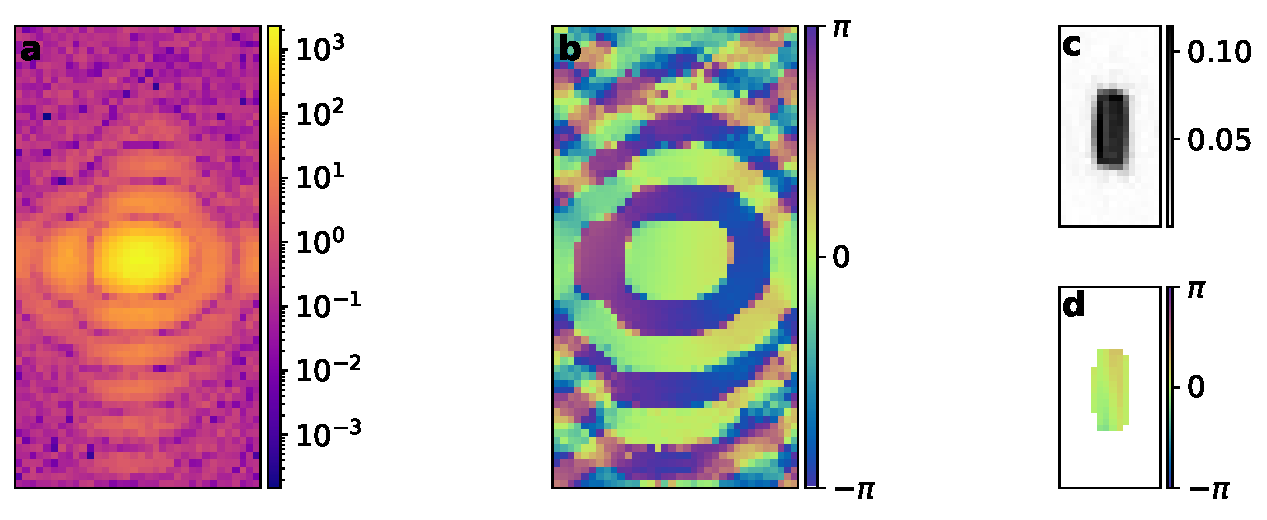
\includegraphics[width=.8\textwidth]{figures/Phasing/rec_space_phase.pdf}
    \caption{Central slice of a typical BCDI pattern (\textbf{a}) with the corresponding RSP (\textbf{b}) obtained after a 
    successful reconstruction of the object (modulus and phase in \textbf{c - d} respectively). It is clear the structural similarity between the diffracted intensity 
    in logarithmic scale and the RSP. Moreover, one can notice that in this case of low strain faceted particle, 
     the RSP varies regularly between 0 and $\pi$ (or $-\pi$) in correspondence of the intensity fringes. }
    \label{fig:rec_space_phase}
\end{figure}

Moreover, given this ``simple'' law of constructive-destructive interferences, we hypothesized the possibility to predict patches 
of this RSP given a portion of diffraction pattern and then, similarly to the inpainting case, stitch together them together
and obtain the full RSP. This entails a number of complications related to the so-called phase symmetries that I have encountered
during the development of the algorithms and that will be discussed in the next sections. \\
Ultimately, the goal of our DL model for phasing is to facilitate the reconstruction of highly strained particles. While 
other works in literature have mostly leveraged the gain in computing time, we aim at tackling those reconstructions for which 
conventional algorithms struggle to find convergence because of the high strain in the particle.   
However, in this case, the aforementioned RSP $\pi$-shifts in between two fringes is much more complicated since the 
strong and extended displacement fields inside the crystal alter the Bragg peak, merging and spreading the fringes 
into an irregularly distributed intensity pattern. \\

% al punto che non si e' in grado di stabilire, a occhio, se l'informazione necessaria per costruire la mappa I-phi e' racchiusa in una porzione 
\section{Dataset creation} 

I have trained our model in a supervised manner, meaning, in our case, that the training was always conducted on simulated data 
only, as the RSP is never experimentally detectable. 
For this reason, I have simulated the training dataset following the same procedure described in Sections 
\ref{sec:dataset_creation2D} and \ref{sec:dataset_creation3D} for the 2D and 3D cases, respectively. However, in this
case, the dataset size was reduced to $64\times64\times64$ pixels, and no gap was applied. Additionally, I have used the 
calculated RSP as the ground truth label for training instead of the masked diffraction pattern.\\

I will anticipate here that for the high strain case I created a dedicated training set simulating the strain by applying 
an artificial ``strong'' phase to the particles. In order to have a diverse population of strain distributions I have 
simulated each object's phase using different functions and parameters, namely: with the sum of two Gaussian functions,
with the sum of two cosine functions and using a random Gaussian distribution. In each case, amplitudes, variances, 
frequencies, and correlation lengths were randomly chosen to ensure a phase variation within the particle ranging between 
$2\pi$ and $5\pi$. By doing this, I could obtain strongly distorted BCDI patterns, similar to experimental high-strain ones. 
In particular, the two Gaussian functions phase can closely emulate the effect of the substrate induced strain inside Winterbottom 
particles. 

\section{2D case low strain}\label{chp:2d_nostrain}
% MODEL 2D CASE NO STRAIN: SHOW THE MODEL PREDICTING THE PHASE AND USE A LOSS ON THE FOURIER TRANSFORM 
Alike the inpainting case, I have first conducted some preliminary studies in 2D, on noise-less low strain data. Here I will 
briefly show the model's architecture, the loss function and the results. 
\subsection{Model structure}
The architecture that I used has a U-Net like structure with an encoder and a decoder. 
The encoder is composed of six convolutional blocks through which the input diffracted intensity is progressively 
reduced from the 64 pixel-side squares to a 1D flattened vector. Each convolutional block is composed of a convolutional 
layer, a LeakyReLU activation function and a MaxPooling layer that halves the feature's map dimensions. (illustrate the 
parameters later). \\
At the end of the encoder the so-called bottleneck composed of a convolutional layer followed by a LeakyReLU activation 
processes the feature map before passing it to the decoder which, by means of transposed convolutions, LeakyReLU activations 
and UpSampling layers, brings back the feature map to the input's size. Skip connections between encoder and decoder blocks 
are employed as well. The output tensor is the result of a last single-channeled convolutional layer activated by a rescaled 
sigmoid. 
This last function in fact has been rescaled onto a $-40\pi$ - $40\pi$ range to allow the prediction of RSP as a continuous 
function, avoiding the $2\pi$-wraps that might cause gradients instabilities. 

\subsection{Input preprocessing} 

Similarly to the inpainting case, the BCDI patterns have been transformed into logarithmic scale and normalized between 
0 and 1. Batches of 32 images at the time were used. 

\subsection{Loss function}
The choice of the loss function was firstly based on what was used in literature. 
A sum of the MSE computed on the objects' moduli and one on the phases has thus been used (Eq. \ref{eq:loss}). The ground truth 
objects were indeed available from the simulated data while the predicted objects have been first calculated with a 2D  
inverse Fourier transform from the diffracted amplitude and the predicted RSP (Eq. \ref{eq:ft_2D}). 
\begin{equation}
    \hat{o}(\mathbf{r})
    \;=\;
    \mathcal{F}^{-1}\!\bigl\{\sqrt{I(\mathbf{q})}\,e^{\,i\,\varphi_{\mathrm{pred}}(\mathbf{q})}\bigr\}(\mathbf{r})
    \quad,
    \label{eq:ft_2D}
\end{equation}

\begin{equation}
    \mathcal{L}
    \;=\;
    \frac{1}{N}\sum_{\mathbf{r}}
    \Bigl(\bigl|\hat{o}(\mathbf{r})\bigr|
        \;-\;\bigl|o(\mathbf{r})\bigr|\Bigr)^{2}
    \;+\;
    \frac{1}{N}\sum_{\mathbf{r}}
    \Bigl(\phi(\mathbf{r})
        \;-\;\phi_{\mathrm{gt}}(\mathbf{r})\Bigr)^{2}
    \quad,
    \label{eq:loss}
\end{equation}
\subsection{Results}
We have conducted the training of the model 8500 simulated BCDI patterns over 30 epochs with a learning rate of 0.0003
and monitored both training and validation loss. Here, Fig.\ref{fig:loss_2mse_nosymm} shows the model's loss during the 
30 epoch long training. However, despite the good decaying trend, typical of proper training, the model does not 
perform optimally when tested on new data. 

\begin{figure}[H]
    \centering
    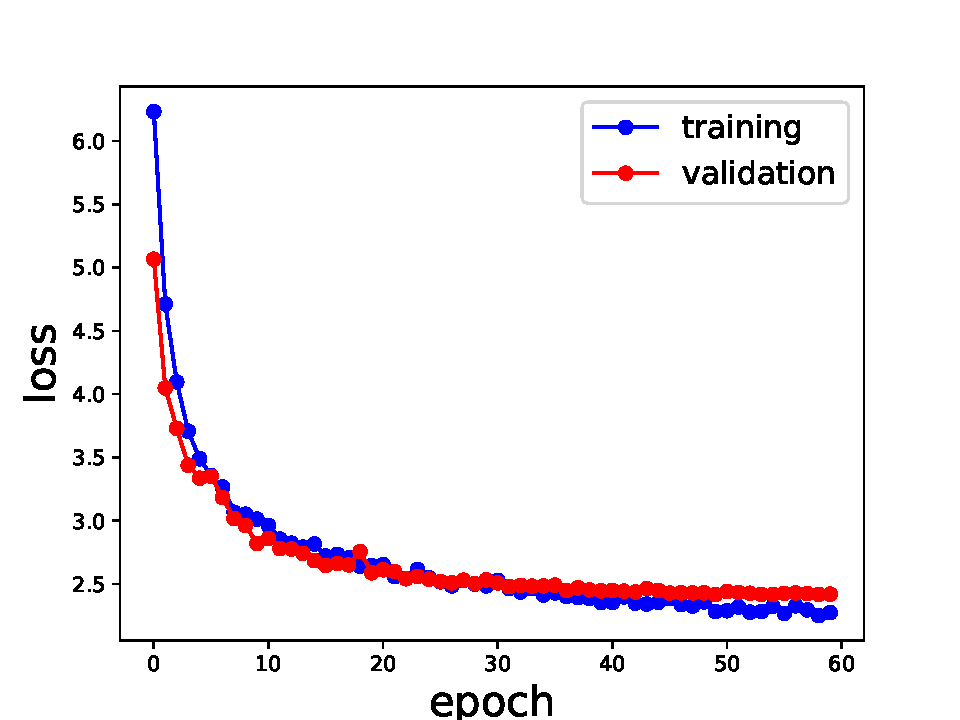
\includegraphics[width=.8\textwidth]{figures/Phasing/loss_low_strain_noiseless_doubleMSE_nosymm.pdf}
    \caption{Training and validation loss over 30 epochs. The curve suggests a proper learning with no overfitting as 
    both losses are decreasing reaching a plateau and the validation loss follows the same trend of the training loss.}
    \label{fig:loss_2mse_nosymm}
\end{figure}

When comparing the reconstructed objects obtained from the predicted RSP with the ground truth ones (Fig. \ref{fig:obj_lowStrain_doubleMSE})
one can draw some interesting conclusions about the model's learning performances. 
First we can observe that the model learns the approximate shape and size of the particle, it produces indeed images 
that resemble the ground truth. The amplitude is concentrated inside the support with little noise outside and the phase 
is overall correct around zero. However, it is also clear that the shape is not quite correct, especially for highly 
non-centrosymmetric objects. For instance, if we consider the object in Fig. \ref{fig:obj_lowStrain_doubleMSE} \textbf{c}, 
we see that the predicted shape seems to be deriving from the incorrect superposition of the correct shape and its 
twin, as well correct. More in general it seems that the model tends to predict centrosymmetric objects, with the tendency
to mix  


\begin{figure}[H]
    \centering
    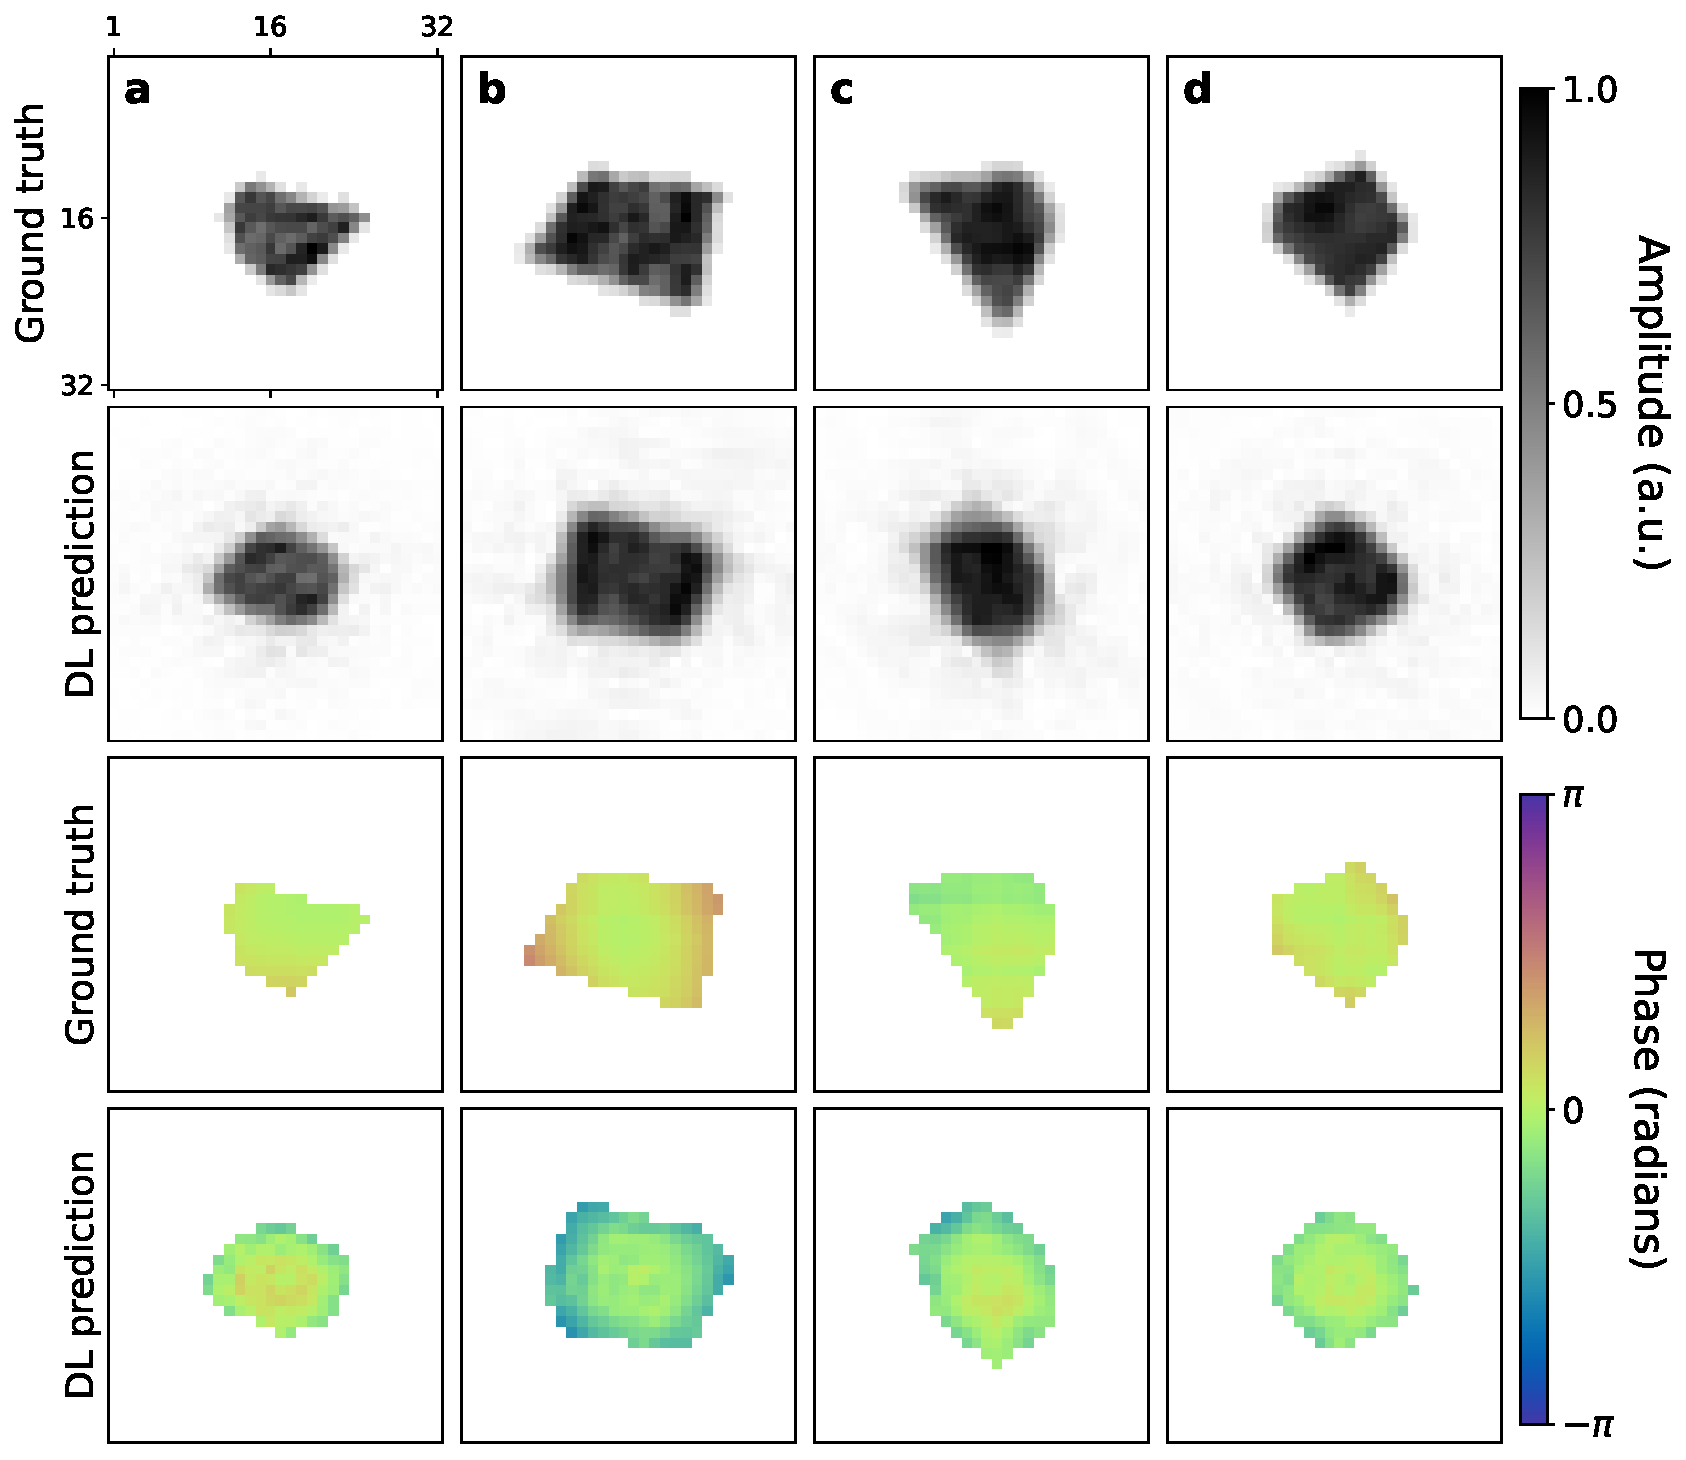
\includegraphics[width=.8\textwidth]{figures/Phasing/obj_low_strain_doubleMSE.pdf}
    \caption{}
    \label{fig:obj_lowStrain_doubleMSE}
\end{figure}

\begin{figure}[H]
    \centering
    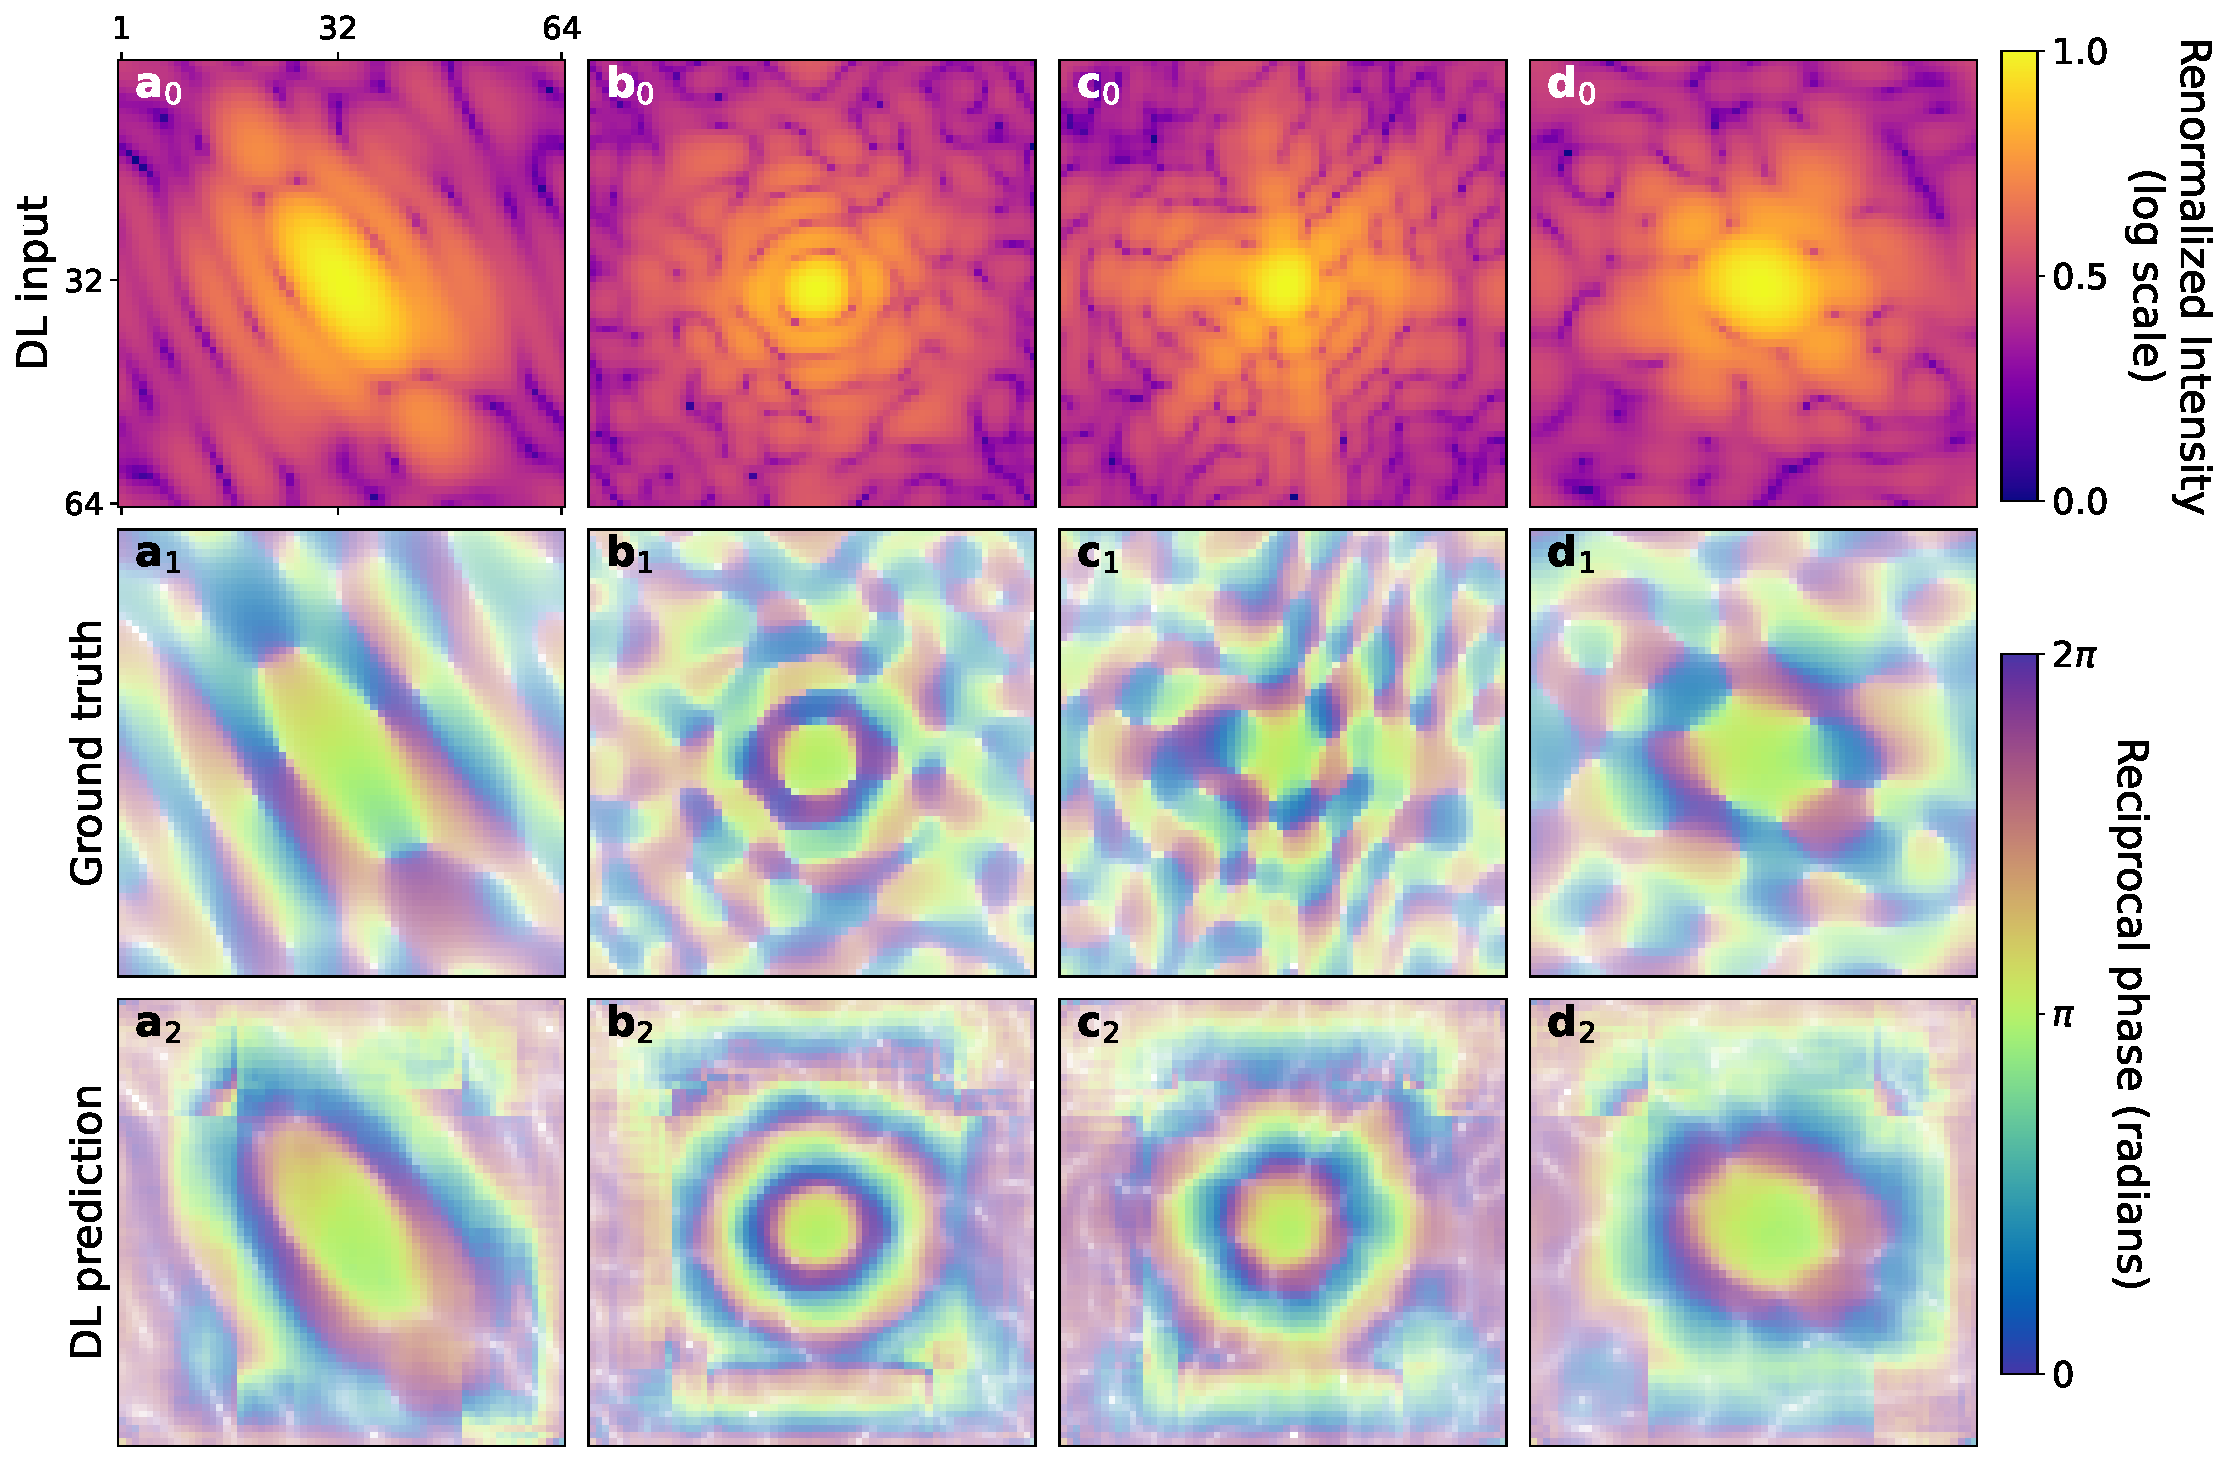
\includegraphics[width=.8\textwidth]{figures/Phasing/RSP_low_strain_doubleMSE.pdf}
    \caption{}
    \label{fig:RSP_lowStrain_doubleMSE}
\end{figure}









\section{Model design: 3D case low strain }\label{chp:3d_nostrain}
% MODEL 3D CASE NO STRAIN: SHOW THE MODEL PREDICTING THE PHASE AND USE A LOSS ON THE FOURIER TRANSFORM 

\section{Patches: 3D case low strain}\label{chp:patches_nostrain}
% MODEL 3D CASE NO STRAIN WITH PATCHES: SHOW THE MODEL WITH DIFFERENT WCA LOSS FUNCTION 


\section{Patches: 3D case high strain}\label{chp:patches_strain}
% MODEL 3D CASE STRAIN WITH PATCHES: SHOW THE FAILURE AND EXPLAIN WHY 

\section{Model design: 3D case high strain }\label{chp:3d_nostrain}
% MODEL 3D CASE STRAIN FULL DIFFRACTION 

\section{Results on 3D case}\label{chp:phasing}
\section{Refinement with iterative algorithms}\label{chp:phasing}
\section{Experimental results}\label{chp:phasing}

